\section{Solution}

\subsection{Mobile Terminal Part}

\subsubsection{Flow Chart}

\hspace*{2em}First the motion of one person is detected by the sensor and become raw data.
   Then the raw data is filtered into acceleration data. 

   The filter mainly did two things.
   One is to abandon the useless data such as temperature and the other is to
   map the acceleration data into float point value between 0 to 5. 

   After that, the acceleration data will be processed through one of the
   following function, matcher and scaler. 

   After the processor, one sound track is created and finally the multiple
   sound tracks are mixed into the final audio. 

\subsubsection{Index Script}

The index script is the one that unity engine recognize and hand over its
control to. 
Thus, we use the index script to get access to the \textbf{physical} part of the
mobile phone, ask for \textbf{memory}, create \textbf{main loop}, and call for
\textbf{matcher} and \textbf{scaler} functions.
The flow chart of the index script is shown in Figure~\ref{indexScript}.

\begin{figure}[htbp]
\centering
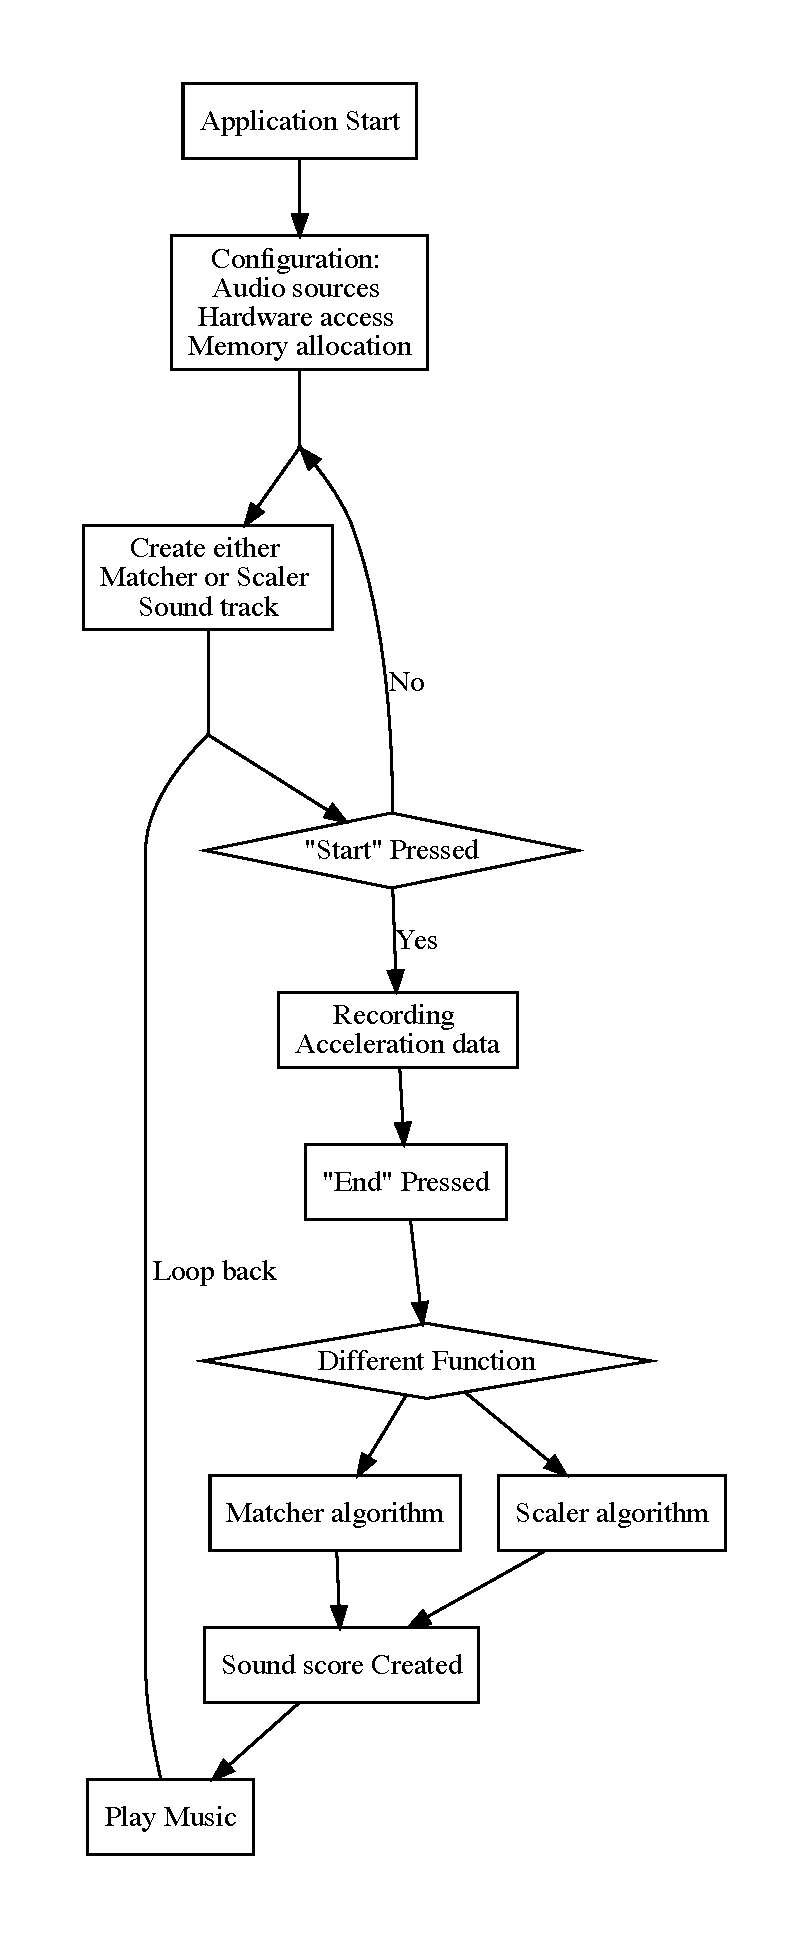
\includegraphics[height=20cm]{figWR/a}
\caption{Flow Chart of the Index Script}
\label{indexScript}
\end{figure}

\subsubsection{Scaler algorithm}

   For the scaler part, also suppose we have the acceleration data.
   Then we separate them into 10 time intervals equally.
   And we find the max value in each interval.
   Then the ruler is created based on the max value and the min value of the
   acceleration data.
   The ruler create 7 blanks vertically for there is 7 tones in one music
   period, which are do re mi...
   Fill in the blank and finally a music score is created and it produces one
   sound track.

   The visual of the scaler process is shown in Figure~\ref{scalerStep}.

\begin{figure}[htbp]
\centering
\newcommand{\widthOfScalerStepFigure}{5cm}
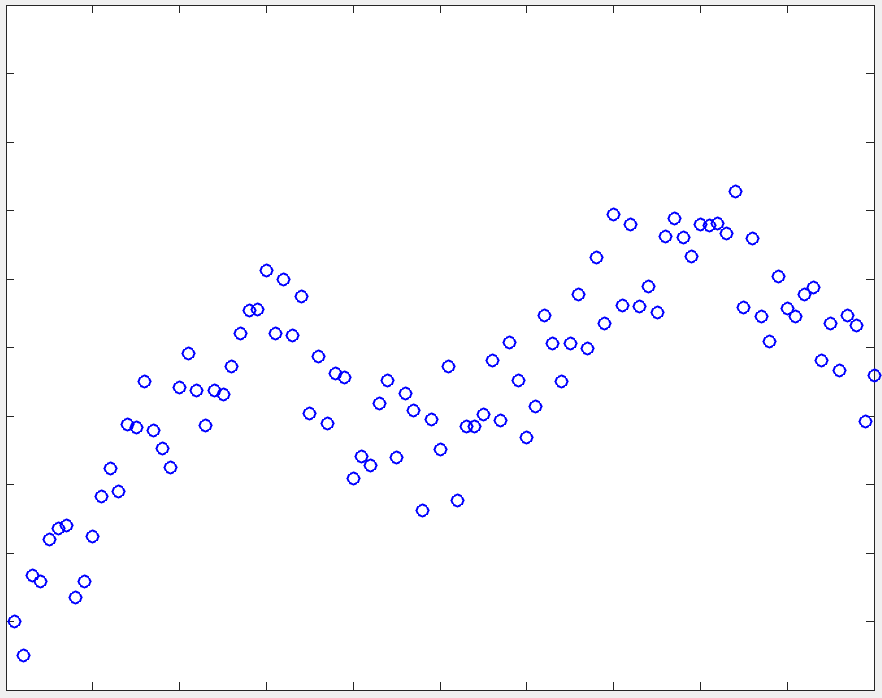
\includegraphics[width=\widthOfScalerStepFigure]{figWR/scaler0}
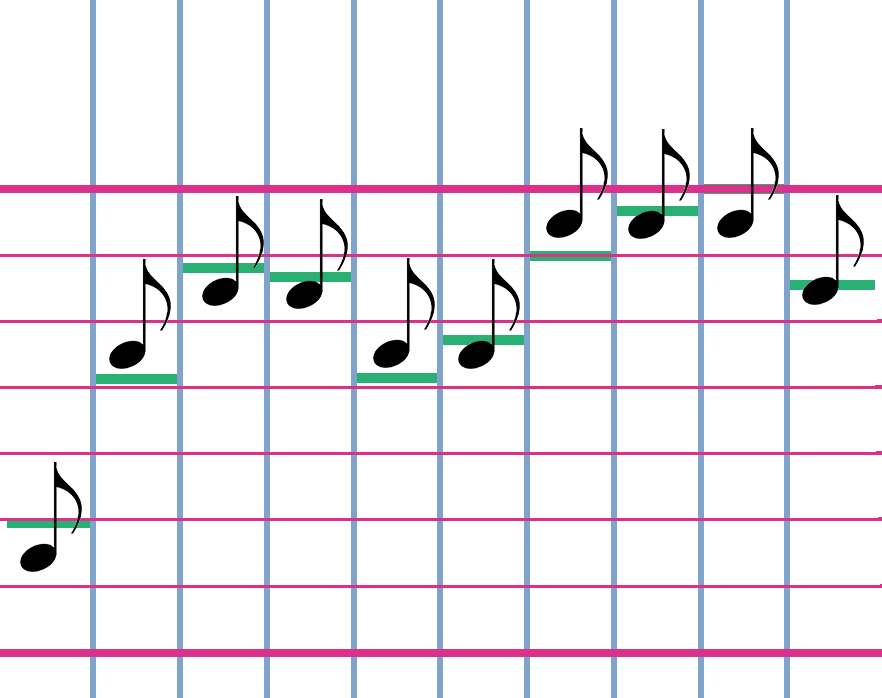
\includegraphics[width=\widthOfScalerStepFigure]{figWR/scaler1}
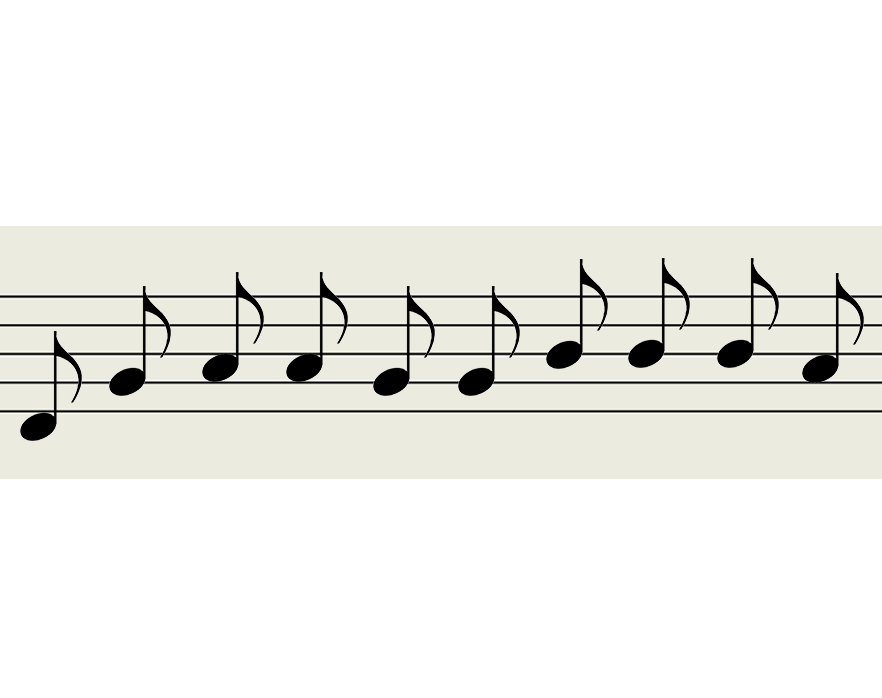
\includegraphics[width=\widthOfScalerStepFigure]{figWR/scaler2}
\caption{Scaler Process}
\label{scalerStep}
\end{figure}

\subsubsection{Matcher algorithm}

   For the matcher part, suppose we have the acceleration data,
   then we compared it with three pre-configured answers,
   calculate the difference between answers and real data.
   The one that has the least sum of absolute value is the audio clip we select.
   Then the corresponding sound track is created.

   The visual of the matcher process is shown in Figure~\ref{matcherStep}.

\begin{figure}[htbp]
\centering
\newcommand{\widthOfMatcherFigure}{8cm}
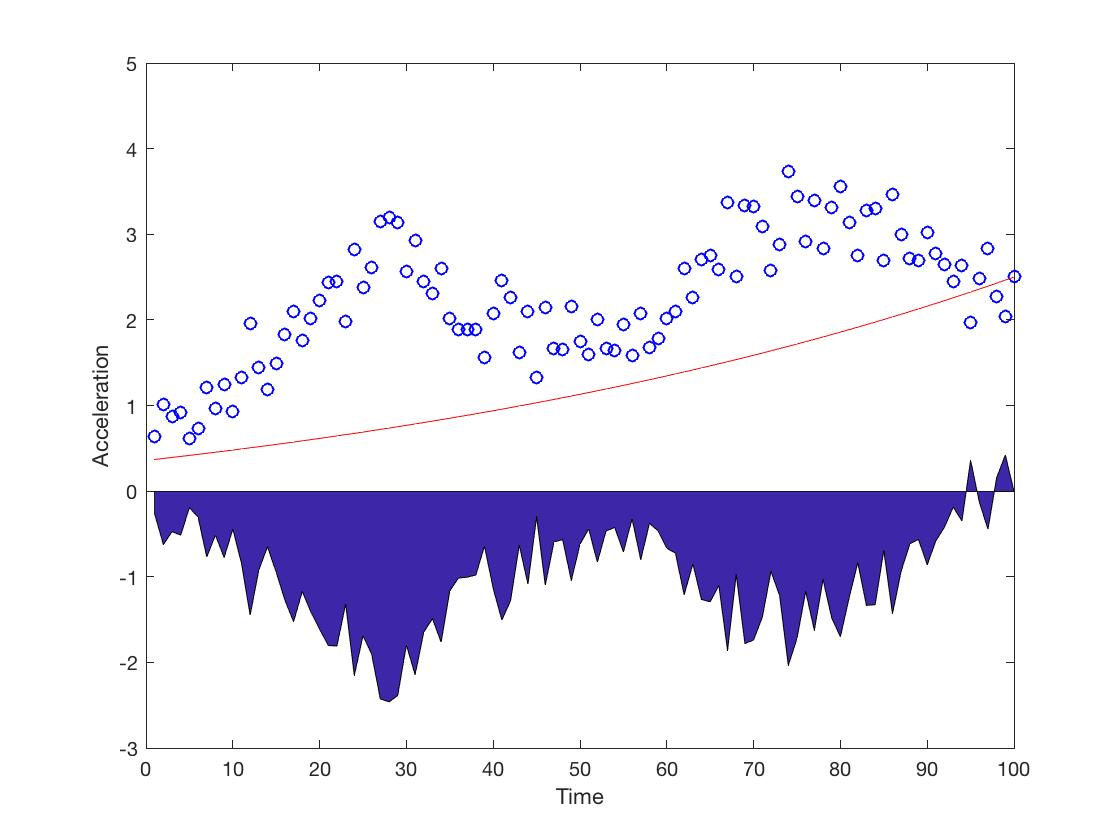
\includegraphics[width=\widthOfMatcherFigure]{figWR/matcher1}
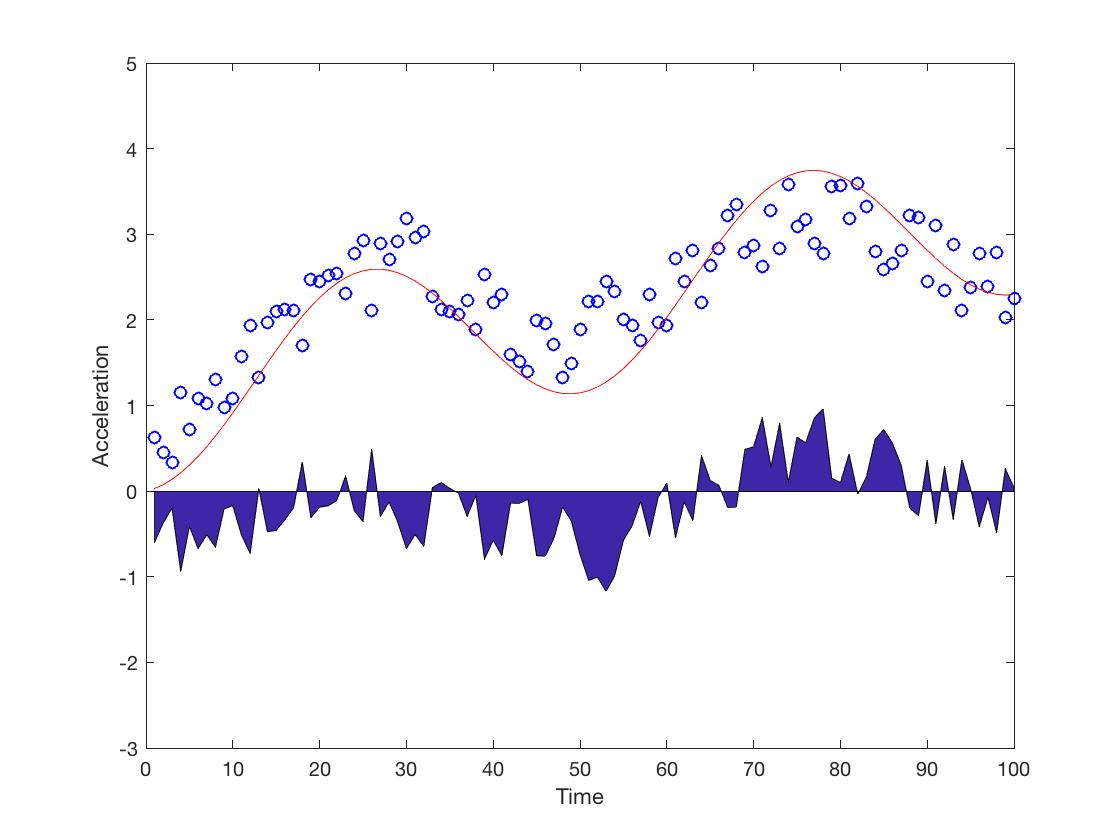
\includegraphics[width=\widthOfMatcherFigure]{figWR/matcher2}
\caption{Matcher Process}
\label{matcherStep}
\end{figure}

\subsubsection{Mixer}

   After we have multiple sound tracks through either of the previous process,
   we mix them together and create the final audio. Feel free to play it.

\subsection{PC Terminal}
\hspace*{2em}Besides the cellphone terminal part, we also designed a PC terminal part, because when users dance, cellphones in hands are not safe enough. Cellphones might be thrown out and hurt someone and then be broken. Moreover, the cellphones are too heavy to carry when doing some fierce action. So developing a safer and lighter bracelet is necessary. The second part of our product can exactly satisfy the needs. \\
\hspace*{2em}The second part consists of a bracelet and a PC terminal. The bracelet contains the sensor JY901, the bluetooth module and batteries. More specifically, the sensor JY901 can detect data, the bluetooth module can transfer data to the terminal and the batteries can power both JY901 and bluetooth. Overall, the bracelet mainly does the detecting job. On the other hand, the PC terminal mainly does the analyzing and generating jobs. The software on PC terminal developed by Unity3D can apply several different algorithm to analyze the data, so that the origin motion kind of the users can be defined. Then by comparing different conditions prepared previously, the software can mix and play all kinds audio source.  \\
\subsubsection{Hardware}
\paragraph{Attitude Sensor JY901}
\hspace*{2em}The sensor JY901 is a attitude sensor that can detect the acceleration, the angle of avertence and angular velocity. The sensor itself consists of three-axis gyroscope, three-axis acceleration sensors, three-axis digital compass and some other motion sensors. The sensor JY901 has the following characteristics:
\begin{itemize}
\item Flexible data outputting ports. (I2C, SPI, TTL are supported)
\item High speed data outputting rate. (Highest 500Hz)
\item Low power consumption. (17mA)
\item Short and stable initializing time. 
\item Support software development. 
\end{itemize}
\paragraph{Bluetooth Module}
\paragraph{Battery}
\paragraph{Fabrication}
\subsubsection{Software}
\paragraph{Data collection algorithm (same with the Mobile terminal part)}
\paragraph{Data transmission algorithm}
\paragraph{ Data analysis algorithm (same with the Mobile terminal part)}
\paragraph{Audio source generating algorithm (same with the Mobile terminal part)}
\subsubsection{Working Principles}